\documentclass[]{elsarticle} %review=doublespace preprint=single 5p=2 column
%%% Begin My package additions %%%%%%%%%%%%%%%%%%%
\usepackage[hyphens]{url}
\usepackage{lineno} % add
\providecommand{\tightlist}{%
  \setlength{\itemsep}{0pt}\setlength{\parskip}{0pt}}

\bibliographystyle{elsarticle-harv}
\biboptions{sort&compress} % For natbib
\usepackage{graphicx}
\usepackage{booktabs} % book-quality tables
%% Redefines the elsarticle footer
%\makeatletter
%\def\ps@pprintTitle{%
% \let\@oddhead\@empty
% \let\@evenhead\@empty
% \def\@oddfoot{\it \hfill\today}%
% \let\@evenfoot\@oddfoot}
%\makeatother

% A modified page layout
\textwidth 6.75in
\oddsidemargin -0.15in
\evensidemargin -0.15in
\textheight 9in
\topmargin -0.5in
%%%%%%%%%%%%%%%% end my additions to header

\usepackage[T1]{fontenc}
\usepackage{lmodern}
\usepackage{amssymb,amsmath}
\usepackage{ifxetex,ifluatex}
\usepackage{fixltx2e} % provides \textsubscript
% use upquote if available, for straight quotes in verbatim environments
\IfFileExists{upquote.sty}{\usepackage{upquote}}{}
\ifnum 0\ifxetex 1\fi\ifluatex 1\fi=0 % if pdftex
  \usepackage[utf8]{inputenc}
\else % if luatex or xelatex
  \usepackage{fontspec}
  \ifxetex
    \usepackage{xltxtra,xunicode}
  \fi
  \defaultfontfeatures{Mapping=tex-text,Scale=MatchLowercase}
  \newcommand{\euro}{€}
\fi
% use microtype if available
\IfFileExists{microtype.sty}{\usepackage{microtype}}{}
\usepackage{longtable}
\usepackage{graphicx}
% We will generate all images so they have a width \maxwidth. This means
% that they will get their normal width if they fit onto the page, but
% are scaled down if they would overflow the margins.
\makeatletter
\def\maxwidth{\ifdim\Gin@nat@width>\linewidth\linewidth
\else\Gin@nat@width\fi}
\makeatother
\let\Oldincludegraphics\includegraphics
\renewcommand{\includegraphics}[1]{\Oldincludegraphics[width=\maxwidth]{#1}}
\ifxetex
  \usepackage[setpagesize=false, % page size defined by xetex
              unicode=false, % unicode breaks when used with xetex
              xetex]{hyperref}
\else
  \usepackage[unicode=true]{hyperref}
\fi
\hypersetup{breaklinks=true,
            bookmarks=true,
            pdfauthor={},
            pdftitle={Short Paper},
            colorlinks=true,
            urlcolor=blue,
            linkcolor=magenta,
            pdfborder={0 0 0}}
\urlstyle{same}  % don't use monospace font for urls
\setlength{\parindent}{0pt}
\setlength{\parskip}{6pt plus 2pt minus 1pt}
\setlength{\emergencystretch}{3em}  % prevent overfull lines
\setcounter{secnumdepth}{0}
% Pandoc toggle for numbering sections (defaults to be off)
\setcounter{secnumdepth}{0}
% Pandoc header


\usepackage[nomarkers]{endfloat}

\begin{document}
\begin{frontmatter}

  \title{Short Paper}
    \author[School of Natural Resources]{Anson Main\corref{c1}}
   \ead{maina@missouri.edu} 
   \cortext[c1]{Corresponding Author}
    \author[School of Natural Resources]{Elisabeth Webb}
   \ead{webbli@missouri.edu} 
  
      \address[Some Institute of Technology]{Department, Street, City, State, Zip}
    \address[Another University]{Department, Street, City, State, Zip}
  
  \begin{abstract}
  This is the abstract.
  
  It consists of two paragraphs.
  \end{abstract}
  
 \end{frontmatter}

\section{Methods}\label{methods}

All analysis were carried away with the R Statistical Software (R Core
Team 2016), all meta-analyses were made on the metafor package
(Viechtbauer 2010). Our estimations were based on the use of
random/mixed-effects models form of meta-analyses, which provide an
unconditional inference about a larger set of studies from which the k
studies included in the meta-analysis are assumed to be a random sample
(L. V. Hedges and Vevea 1998). This estimations do not assume that this
larger set consists only of studies that have actually been conducted,
but instead envision a hypothetical population of studies that comprises
studies that have been conducted, that could have been conducted, or
that may be conducted in the future (L. V. Hedges and Vevea 1998).

We used the \emph{escalc} function of the metafor package to estimate
the effect size estimates (Viechtbauer 2010), we used the
\emph{standardized mean difference with heteroscedastic population
variances in the two groups} (SDMH) as our estimator for effect size
(Bonett 2009), the metafor package also corrects the slight positive
bias of the estimation following (Wasserman, Hedges, and Olkin 1988). To
be extra conservative we used the unbiased estimates of the sampling
variances. In all cases the residual heterogeneity estimator was Hedges.

Since we used mixed effect models we used the The Knapp and Hartung
adjustment \textbf{(Knapp and Hartung, 2003)} to test the individual
coefficients of the model.

\subsection{Test for (Residual)
Heterogeneity}\label{test-for-residual-heterogeneity}

For each model we tested for residual heterogeneity, if we used models
without moderators, then the Cochran's Q-test (Cochran 1954) was used to
test whether the variability in the observed effect sizes or outcomes is
larger than would be expected based on sampling variability alone.
\emph{A significant test suggests that the true effects or outcomes are
heterogeneous}. When moderators were included in the models the
Q\_E-test for residual heterogeneity was used, this tests whether the
variability in the observed effect sizes or outcomes not accounted for
by the moderators included in the model is larger than would be expected
based on sampling variability alone. When using moderators to explain
more variability a pseudo R squared was computed following (Raudenbush
2009).

\section{Results}\label{results}

As we can see in figure 1, the most common type of performance measured
in studies was abundance, with 101 estimations, followed by reproduction
with 44 estimation, behavior with 23, and finally survival and condition
with 16 each.

\begin{figure}[htbp]
\centering
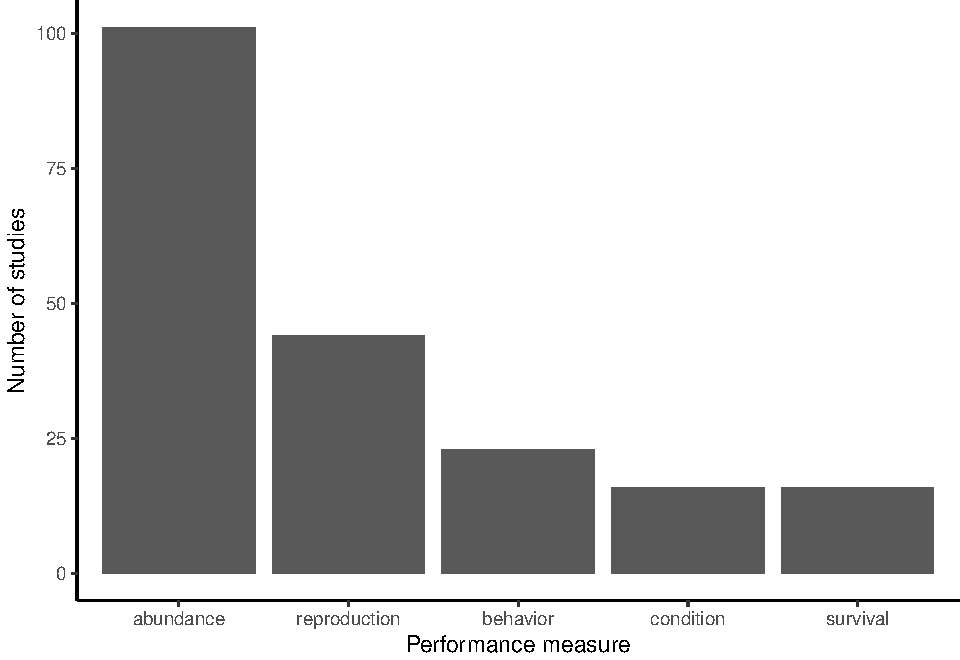
\includegraphics{MetanalysisNeonics_files/figure-latex/unnamed-chunk-2-1.pdf}
\caption{Number of estimation of effect size within the meta-analyses}
\end{figure}

\begin{longtable}[c]{@{}rrrlrrrr@{}}
\caption{effect size of the Standardized mean difference for each type
of estimation of performance, it's standard error and
p-value}\tabularnewline
\toprule
estimate & ci.ub & ci.lb & group & p & n & I2 & pvalCT\tabularnewline
\midrule
\endfirsthead
\toprule
estimate & ci.ub & ci.lb & group & p & n & I2 & pvalCT\tabularnewline
\midrule
\endhead
-0.917 & -0.423 & -1.410 & Abundance & 0.000 & 101 & 90.594 &
0\tabularnewline
-2.508 & 0.940 & -5.957 & Behavior & 0.154 & 23 & 99.742 &
0\tabularnewline
-5.319 & -1.556 & -9.083 & Survival & 0.006 & 16 & 98.756 &
0\tabularnewline
-3.366 & 13.710 & -20.441 & Reproduction & 0.699 & 44 & 99.995 &
0\tabularnewline
-1.078 & -0.128 & -2.027 & Condition & 0.026 & 16 & 98.597 &
0\tabularnewline
\bottomrule
\end{longtable}

\subsection{Overall effect size}\label{overall-effect-size}

As we can see in table 1 and figure 2, all estimations of the effects
are negative. However, only abundance, survival and condition have
significative negative effects. Survival has the highest effect size,
with a mean difference estimation of -5.32

\begin{figure}[htbp]
\centering
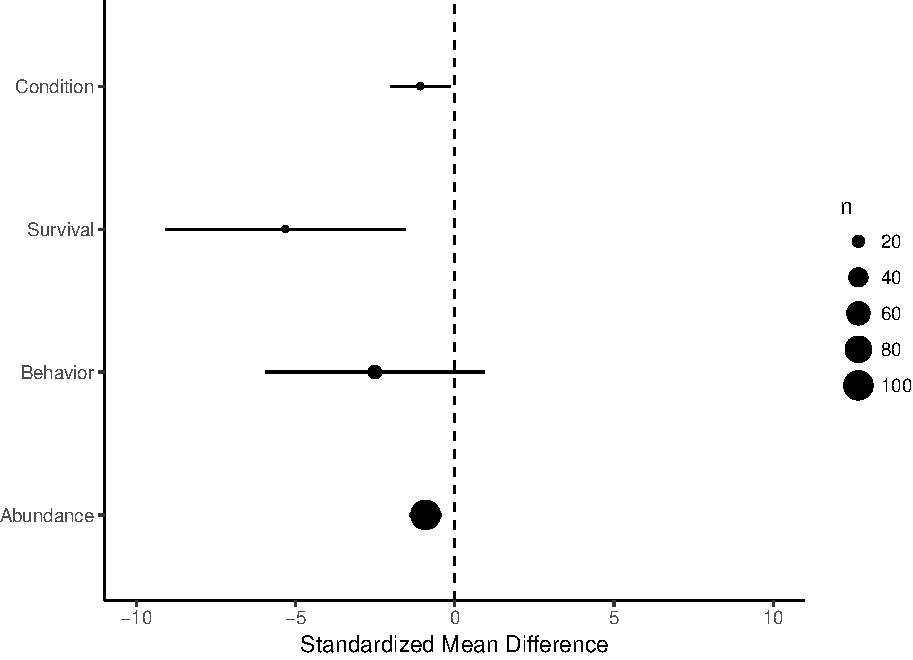
\includegraphics{MetanalysisNeonics_files/figure-latex/unnamed-chunk-4-1.pdf}
\caption{effect size of the Standardized mean difference for each type
of estimation of performance and it's standard error}
\end{figure}

\section{Estimations using
moderators:}\label{estimations-using-moderators}

\section{Abundance}\label{abundance}

\begin{figure}[htbp]
\centering
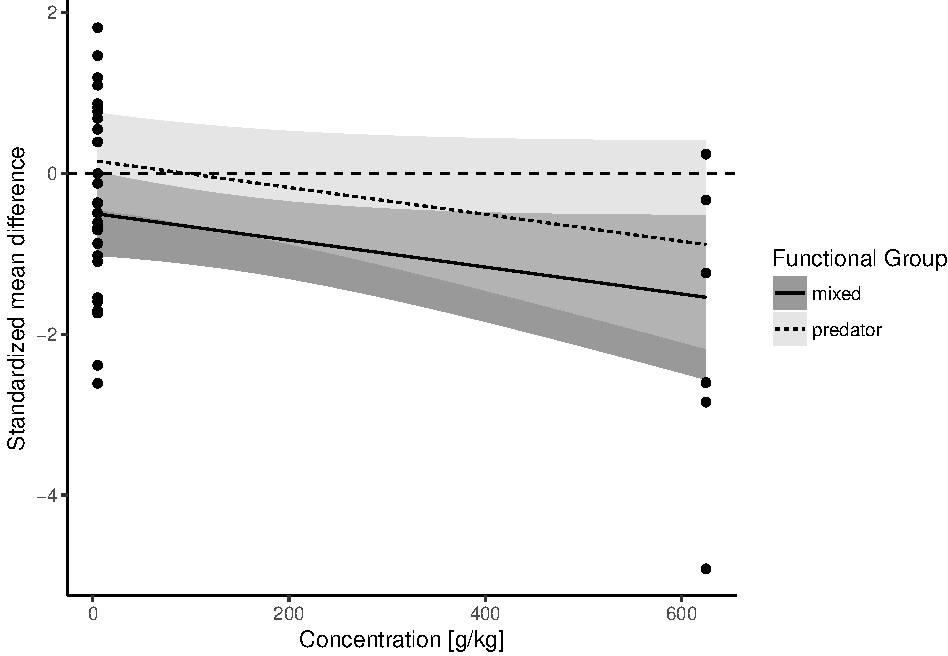
\includegraphics{MetanalysisNeonics_files/figure-latex/unnamed-chunk-10-1.pdf}
\caption{effect size of the Standardized mean difference of Abundance
and concentration {[}g/Kg{]}}
\end{figure}

\subsubsection{Comparison of models}\label{comparison-of-models}

\begin{longtable}[c]{@{}lrrrrr@{}}
\caption{Comparison of models taking into account p value, Pseudo R
squared and AICc}\tabularnewline
\toprule
model & p\_value & R\_squared & AICc & deltaAICc & Weight\tabularnewline
\midrule
\endfirsthead
\toprule
model & p\_value & R\_squared & AICc & deltaAICc & Weight\tabularnewline
\midrule
\endhead
y \textasciitilde{} Concentration {[}g/kg{]} + Nesting Area + Functional
Group & 0.013 & 0.37 & 132.095 & 0.000 & 0.363\tabularnewline
y \textasciitilde{} Concentration {[}g/kg{]} + Functional group & 0.017
& 0.32 & 132.421 & 0.326 & 0.309\tabularnewline
y \textasciitilde{} Concentration {[}g/kg{]} & 0.019 & 0.27 & 132.915 &
0.820 & 0.241\tabularnewline
y \textasciitilde{} Concentration {[}g/kg{]} + Nesting Area & 0.052 &
0.26 & 134.968 & 2.872 & 0.086\tabularnewline
y \textasciitilde{} Concentration {[}kg/ha{]} + Nesting Area +
Functional Group & 0.019 & 0.36 & 164.602 & 32.507 &
0.000\tabularnewline
y \textasciitilde{} Concentration {[}Kg/Ha{]} & 0.165 & 0.04 & 164.902 &
32.807 & 0.000\tabularnewline
y \textasciitilde{} 1 & 0.000 & 0.00 & 463.583 & 331.488 &
0.000\tabularnewline
y \textasciitilde{} Functional group & 0.106 & 0.06 & 464.017 & 331.922
& 0.000\tabularnewline
y \textasciitilde{} Nesting Area & 0.532 & 0.00 & 466.648 & 334.553 &
0.000\tabularnewline
y \textasciitilde{} Order + Functional group & 0.028 & 0.17 & 472.253 &
340.158 & 0.000\tabularnewline
\bottomrule
\end{longtable}

\section{Behaviour}\label{behaviour}

\begin{figure}[htbp]
\centering
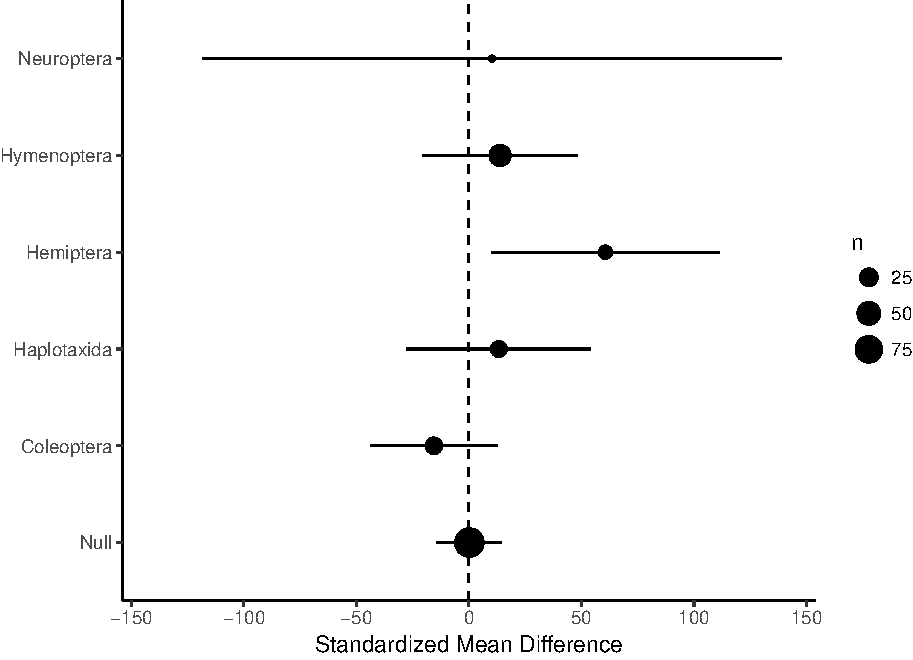
\includegraphics{MetanalysisNeonics_files/figure-latex/unnamed-chunk-18-1.pdf}
\caption{effect size of the Standardized mean difference of behavior and
concentration (ppb)}
\end{figure}

\begin{figure}[htbp]
\centering
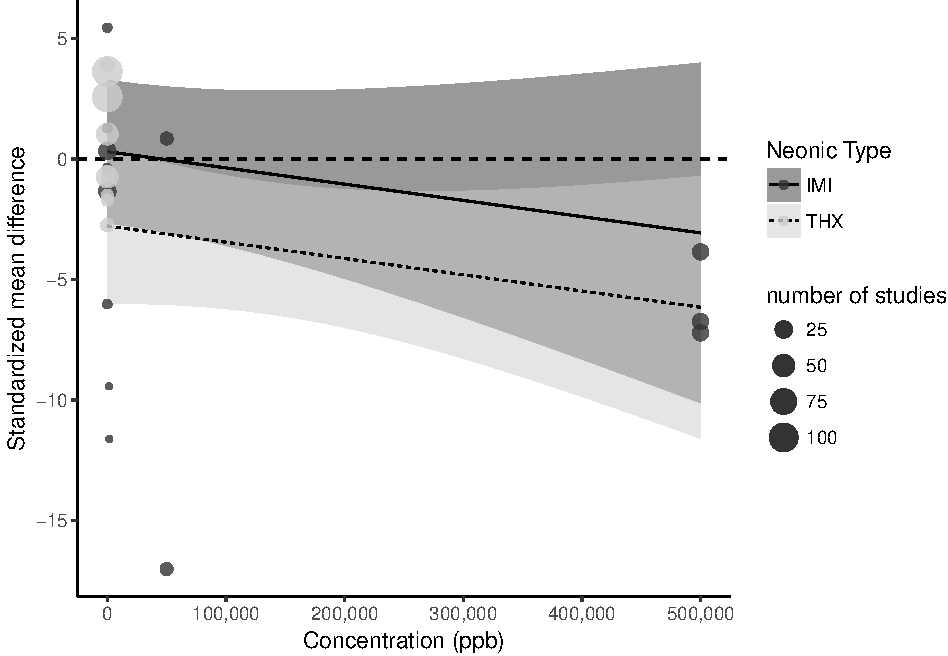
\includegraphics{MetanalysisNeonics_files/figure-latex/unnamed-chunk-20-1.pdf}
\caption{effect size of the concentration and neonic type on the
behavior Standardized mean difference of abundance}
\end{figure}

\subsubsection{Comparison of models}\label{comparison-of-models-1}

\begin{longtable}[c]{@{}lrrrrr@{}}
\caption{Comparison of models taking into account p value, Pseudo R
squared and AICc}\tabularnewline
\toprule
model & p\_value & R\_squared & AICc & deltaAICc & Weight\tabularnewline
\midrule
\endfirsthead
\toprule
model & p\_value & R\_squared & AICc & deltaAICc & Weight\tabularnewline
\midrule
\endhead
y \textasciitilde{} Concentration {[}ppb{]} & 0.107 & 0.05 & 142.911 &
0.000 & 0.54\tabularnewline
y \textasciitilde{} Concentration + neonic type & 0.090 & 0.15 & 143.231
& 0.320 & 0.46\tabularnewline
y \textasciitilde{} study type & 0.110 & 0.08 & 166.687 & 23.776 &
0.00\tabularnewline
y \textasciitilde{} neonic type & 0.181 & 0.04 & 167.467 & 24.556 &
0.00\tabularnewline
y \textasciitilde{} Treatment type & 0.460 & 0.00 & 170.758 & 27.847 &
0.00\tabularnewline
y \textasciitilde{} Treatment type + Functional group & 0.375 & 0.02 &
175.035 & 32.124 & 0.00\tabularnewline
\bottomrule
\end{longtable}

\section{Reproduction}\label{reproduction}

\begin{figure}[htbp]
\centering
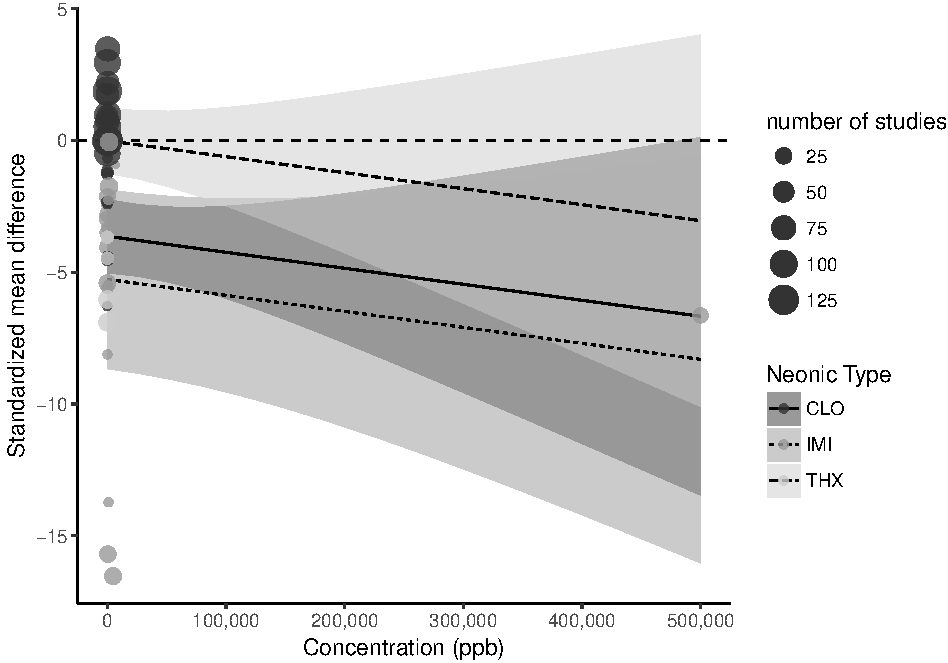
\includegraphics{MetanalysisNeonics_files/figure-latex/unnamed-chunk-29-1.pdf}
\caption{effect size of the concentration and neonic type on the
reporoduction Standardized mean difference of abundance}
\end{figure}

\subsubsection{Comparison of models}\label{comparison-of-models-2}

\begin{longtable}[c]{@{}lrrrrr@{}}
\caption{Comparison of models taking into account p value, Pseudo R
squared and AICc}\tabularnewline
\toprule
model & p\_value & R\_squared & AICc & deltaAICc & Weight\tabularnewline
\midrule
\endfirsthead
\toprule
model & p\_value & R\_squared & AICc & deltaAICc & Weight\tabularnewline
\midrule
\endhead
y \textasciitilde{} Concentration {[}ppb{]} + Neonic type & 0.000 & 0.43
& 213.923 & 0.000 & 1\tabularnewline
y \textasciitilde{} Concentration {[}ppb{]} & 0.194 & 0.01 & 235.285 &
21.362 & 0\tabularnewline
y \textasciitilde{} Order + Nesting Area & 0.940 & 0.00 & 471.357 &
257.434 & 0\tabularnewline
y \textasciitilde{} Order + Functional group & 0.513 & 0.08 & 476.834 &
262.912 & 0\tabularnewline
\bottomrule
\end{longtable}

\section*{References}\label{references}
\addcontentsline{toc}{section}{References}

Bonett, Douglas G. 2009. ``Meta-Analytic Interval Estimation for
Standardized and Unstandardized Mean Differences.'' \emph{Psychological
Methods} 14 (3). American Psychological Association: 225.

Cochran, William G. 1954. ``The Combination of Estimates from Different
Experiments.'' \emph{Biometrics} 10 (1). JSTOR: 101--29.

Hedges, Larry V, and Jack L Vevea. 1998. ``Fixed-and Random-Effects
Models in Meta-Analysis.'' \emph{Psychological Methods} 3 (4). American
Psychological Association: 486.

R Core Team. 2016. \emph{R: A Language and Environment for Statistical
Computing}. Vienna, Austria: R Foundation for Statistical Computing.
\url{https://www.R-project.org/}.

Raudenbush, Stephen W. 2009. ``Analyzing Effect Sizes: Random-Effects
Models.'' \emph{The Handbook of Research Synthesis and Meta-Analysis} 2:
295--316.

Viechtbauer, Wolfgang. 2010. ``Conducting Meta-Analyses in R with the
metafor Package.'' \emph{Journal of Statistical Software} 36 (3): 1--48.
\url{http://www.jstatsoft.org/v36/i03/}.

Wasserman, Stanley, Larry V. Hedges, and Ingram Olkin. 1988.
``Statistical Methods for Meta-Analysis.'' \emph{Journal of Educational
Statistics} 13 (1). JSTOR: 75.
doi:\href{http://dx.doi.org/10.2307/1164953}{10.2307/1164953}.

\end{document}


